\documentclass[tikz,border=5pt]{standalone}
\usepackage{amsmath}
\begin{document}

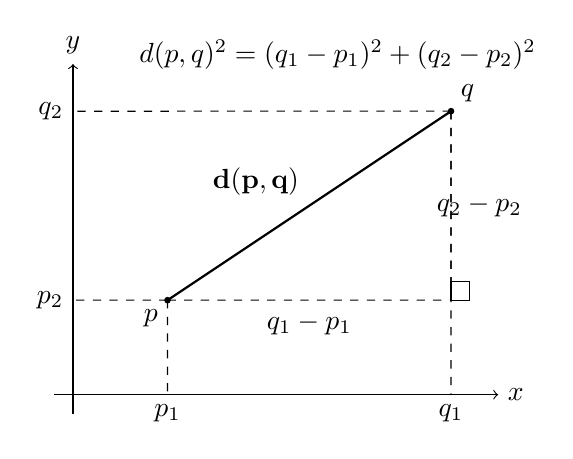
\begin{tikzpicture}[scale=1.2]
  % Axes
  \draw[->] (-0.2,0) -- (4.5,0) node[right] {$x$};
  \draw[->] (0,-0.2) -- (0,3.5) node[above] {$y$};

  % Points
  \coordinate (p) at (1,1);
  \coordinate (q) at (4,3);

  % Dashed lines
  \draw[dashed] (p) -- (1,0) node[below] {$p_1$};
  \draw[dashed] (p) -- (0,1) node[left] {$p_2$};
  \draw[dashed] (q) -- (4,0) node[below] {$q_1$};
  \draw[dashed] (q) -- (0,3) node[left] {$q_2$};
  \draw[dashed] (p) -- (4,1);
  \draw[dashed] (q) -- (4,1);

  % Right angle marker
  \draw (4,1) rectangle +(0.2,0.2);

  % Line between points
  \draw[thick] (p) -- (q) node[midway, above left] {$\mathbf{d(p,q)}$};

  % Labels for p and q
  \fill (p) circle (1pt) node[below left] {$p$};
  \fill (q) circle (1pt) node[above right] {$q$};

  % Difference labels
  \node at (2.5,0.75) {$q_1 - p_1$};
  \node at (4.3,2) {$q_2 - p_2$};

  % Equation on top
  \node[align=center] at (2.8,3.6)
  {$d(p,q)^2 = (q_1 - p_1)^2 + (q_2 - p_2)^2$};

\end{tikzpicture}

\end{document}
